%*******************************************************
% outside of back cover
%*******************************************************

\newgeometry{centering,margin=2.5cm}
\thispagestyle{empty}
\pagecolor{black}\afterpage{\nopagecolor}

\backgroundsetup{
scale=1,
color=black,
opacity=0.3,
angle=0,
contents={%
%   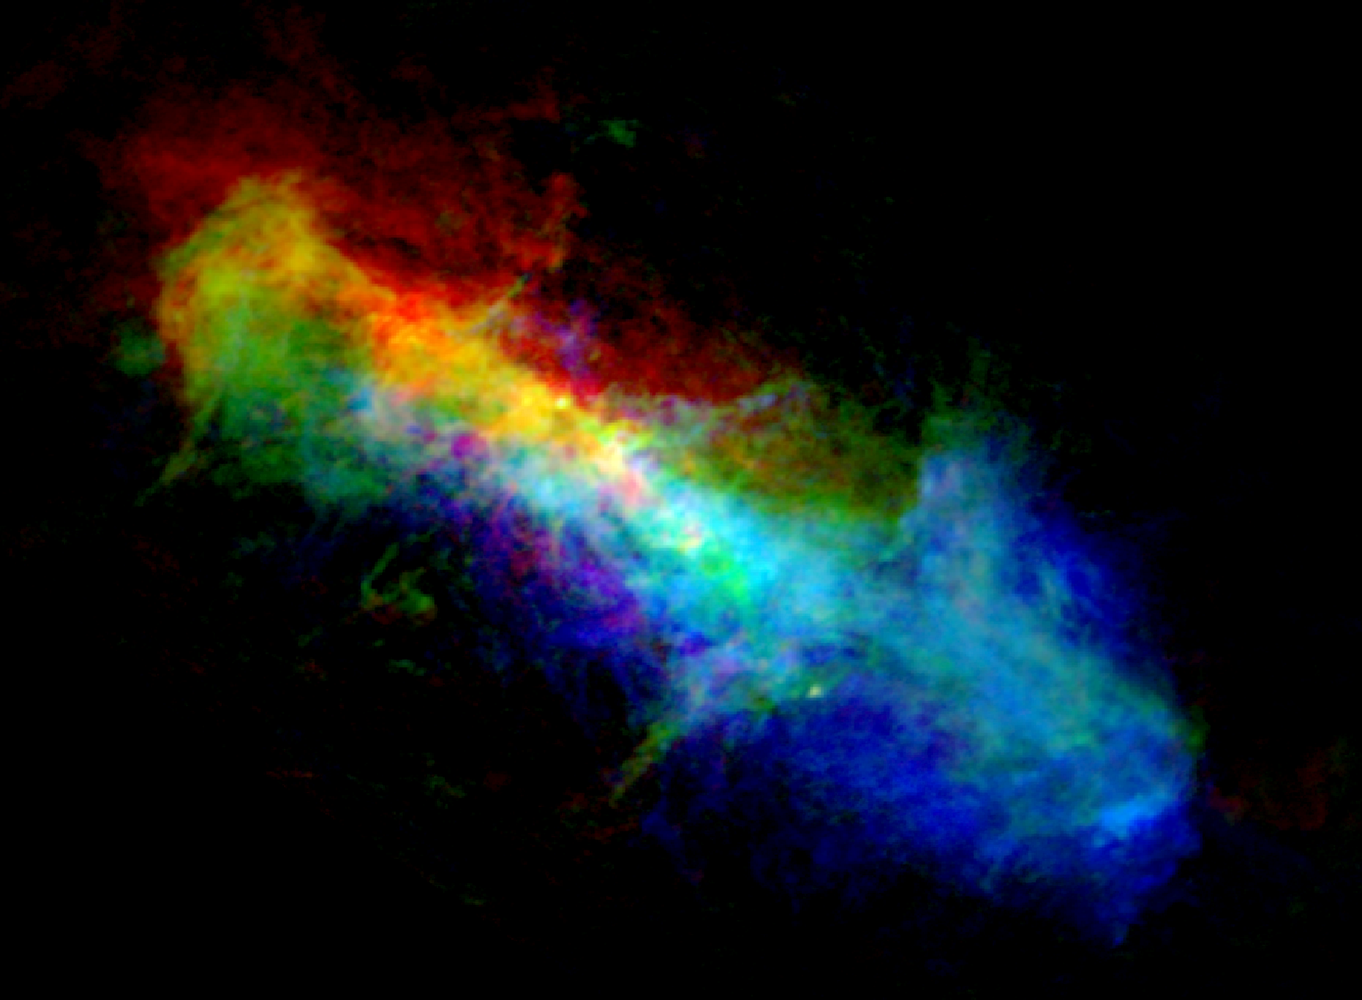
\includegraphics[width=\paperwidth]{thesis/images/frontmatter/cover.png}
  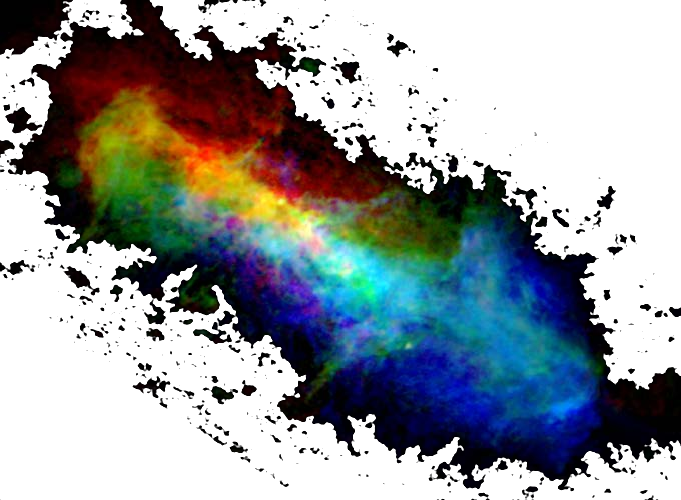
\includegraphics[width=\paperwidth]{thesis/images/frontmatter/cover2.pdf}
  }%
}
\BgThispage

{
\color{white}
\vspace*{-1cm}

Starburst galaxies are characterized by intense star formation at high star formation rate surface densities and short gas depletion times. 
Strong stellar feedback drives galaxy-scale winds and outflows in all gas phases, i.e. ionized, neutral and molecular.
The extreme conditions in local starburst galaxies are thought to be similar to those in typical high-redshift star forming galaxies, e.g. at the peak of the cosmic star formation history.
Since those distant galaxies cannot be studied at the required parsec scale resolution, only local starbursts allow us to study the high activity mode of star formation and related feedback processes that were prevalent over much of the universe's past.

In this thesis, we present and analyze very high resolution (0.15\arcsec or $\sim2.5$\,pc) ALMA observations of the nuclear starburst in \ngc253. 
Using this data, we study the molecular outflow in unprecedented detail, zoom into \ngc253's super star clusters and compare the starburst to the similar but more quiescent center of the Milky Way.
}

\clearpage
\restoregeometry
